%
% hilfstabellen.tex
% Autor: Michael Steiner
%
% (c) 2020 Prof Dr Andreas Müller, Hochschule Rapperswil
%
\section{$\mathbb{F}_{11}$ Hilfstabellen
	\label{reedsolomon:section:hilfstabellen}}
\rhead{Hilfstabellen}

\textbf{TODO}: gibt es eine besser darstellungsart der tabellen? (\& platzierung der subsections)

Um das rechnen  zu erleichtern findet man in diesem Abschnitt die Resultate, die bei der Addition und der Multiplikation in $\mathbb{F}_{11}$ resultieren.

\subsection{Additionstabelle
	\label{reedsolomon:subsection:adtab}}	
% created by Michael Steiner
%
% Restetabelle von F_11: Addition

% alternatives design
%\begin{figure}
%\begin{center}
%\begin{tabular}{|>{$}c<{$}|>{$}c<{$}>{$}c<{$}>{$}c<{$}>{$}c<{$}>{$}c<{$}>{$}c<{$}>{$}c<{$}>{$}c<{$}>{$}c<{$}>{$}c<{$}>{$}c<{$}|}
%\hline
%+&0&1&2&3&4&5&6&7&8&9&10\\
%\hline
%0&0&1&2&3&4&5&6&7&8&9&10\\
%1&1&2&3&4&5&6&7&8&9&10&0\\
%2&2&3&4&5&6&7&8&9&10&0&1\\
%3&3&4&5&6&7&8&9&10&0&1&2\\
%4&4&5&6&7&8&9&10&0&1&2&3\\
%5&5&6&7&8&9&10&0&1&2&3&4\\
%6&6&7&8&9&10&0&1&2&3&4&5\\
%7&7&8&9&10&0&1&2&3&4&5&6\\
%8&8&9&10&0&1&2&3&4&5&6&7\\
%9&9&10&0&1&2&3&4&5&6&7&8\\
%10&10&0&1&2&3&4&5&6&7&8&9\\
%\hline
%\end{tabular}
%\end{center}
%\end{figure}

\begin{center}

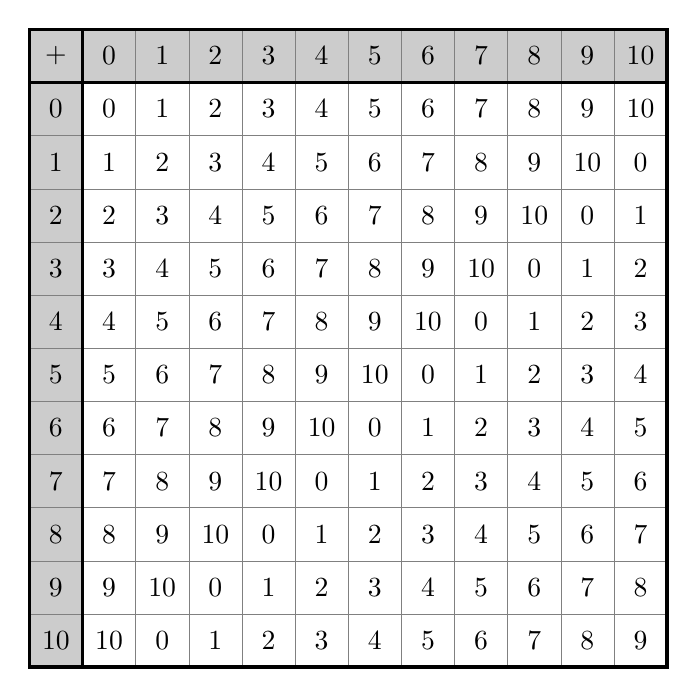
\begin{tikzpicture}[>=latex,thick,scale=0.45]
\fill[color=gray!40] (0,0) rectangle (18,-1.5);
\fill[color=gray!40] (0,0) rectangle (1.5,-18);	
\draw[step = 1.5, gray,very thin] (0,0) grid (18,-18);
\draw[very thick] (0,0) rectangle (18,-18);
\draw[very thick] (0,-1.5) -- (18,-1.5);
\draw[very thick] (1.5,0) -- (1.5,-18);
\node at (0.75,-0.75) {$+$};
\foreach \x in {0,...,10}
	\node at (2.25+\x*1.5,-0.75) {$\x$};
\foreach \y in {0,...,10}
	\node at (0.75,-2.25+\y*-1.5) {$\y$};
% Row 0
\node at ( 2.25,-2.25) {$0$};
\node at ( 3.75,-2.25) {$1$};
\node at ( 5.25,-2.25) {$2$};
\node at ( 6.75,-2.25) {$3$};
\node at ( 8.25,-2.25) {$4$};
\node at ( 9.75,-2.25) {$5$};
\node at (11.25,-2.25) {$6$};
\node at (12.75,-2.25) {$7$};
\node at (14.25,-2.25) {$8$};
\node at (15.75,-2.25) {$9$};
\node at (17.25,-2.25) {$10$};
% Row 1
\node at ( 2.25,-3.75) {$1$};
\node at ( 3.75,-3.75) {$2$};
\node at ( 5.25,-3.75) {$3$};
\node at ( 6.75,-3.75) {$4$};
\node at ( 8.25,-3.75) {$5$};
\node at ( 9.75,-3.75) {$6$};
\node at (11.25,-3.75) {$7$};
\node at (12.75,-3.75) {$8$};
\node at (14.25,-3.75) {$9$};
\node at (15.75,-3.75) {$10$};
\node at (17.25,-3.75) {$0$};
% Row 2
\node at ( 2.25,-5.25) {$2$};
\node at ( 3.75,-5.25) {$3$};
\node at ( 5.25,-5.25) {$4$};
\node at ( 6.75,-5.25) {$5$};
\node at ( 8.25,-5.25) {$6$};
\node at ( 9.75,-5.25) {$7$};
\node at (11.25,-5.25) {$8$};
\node at (12.75,-5.25) {$9$};
\node at (14.25,-5.25) {$10$};
\node at (15.75,-5.25) {$0$};
\node at (17.25,-5.25) {$1$};
% Row 3
\node at ( 2.25,-6.75) {$3$};
\node at ( 3.75,-6.75) {$4$};
\node at ( 5.25,-6.75) {$5$};
\node at ( 6.75,-6.75) {$6$};
\node at ( 8.25,-6.75) {$7$};
\node at ( 9.75,-6.75) {$8$};
\node at (11.25,-6.75) {$9$};
\node at (12.75,-6.75) {$10$};
\node at (14.25,-6.75) {$0$};
\node at (15.75,-6.75) {$1$};
\node at (17.25,-6.75) {$2$};
% Row 4
\node at ( 2.25,-8.25) {$4$};
\node at ( 3.75,-8.25) {$5$};
\node at ( 5.25,-8.25) {$6$};
\node at ( 6.75,-8.25) {$7$};
\node at ( 8.25,-8.25) {$8$};
\node at ( 9.75,-8.25) {$9$};
\node at (11.25,-8.25) {$10$};
\node at (12.75,-8.25) {$0$};
\node at (14.25,-8.25) {$1$};
\node at (15.75,-8.25) {$2$};
\node at (17.25,-8.25) {$3$};
% Row 5
\node at ( 2.25,-9.75) {$5$};
\node at ( 3.75,-9.75) {$6$};
\node at ( 5.25,-9.75) {$7$};
\node at ( 6.75,-9.75) {$8$};
\node at ( 8.25,-9.75) {$9$};
\node at ( 9.75,-9.75) {$10$};
\node at (11.25,-9.75) {$0$};
\node at (12.75,-9.75) {$1$};
\node at (14.25,-9.75) {$2$};
\node at (15.75,-9.75) {$3$};
\node at (17.25,-9.75) {$4$};
% Row 6
\node at ( 2.25,-11.25) {$6$};
\node at ( 3.75,-11.25) {$7$};
\node at ( 5.25,-11.25) {$8$};
\node at ( 6.75,-11.25) {$9$};
\node at ( 8.25,-11.25) {$10$};
\node at ( 9.75,-11.25) {$0$};
\node at (11.25,-11.25) {$1$};
\node at (12.75,-11.25) {$2$};
\node at (14.25,-11.25) {$3$};
\node at (15.75,-11.25) {$4$};
\node at (17.25,-11.25) {$5$};
% Row 7
\node at ( 2.25,-12.75) {$7$};
\node at ( 3.75,-12.75) {$8$};
\node at ( 5.25,-12.75) {$9$};
\node at ( 6.75,-12.75) {$10$};
\node at ( 8.25,-12.75) {$0$};
\node at ( 9.75,-12.75) {$1$};
\node at (11.25,-12.75) {$2$};
\node at (12.75,-12.75) {$3$};
\node at (14.25,-12.75) {$4$};
\node at (15.75,-12.75) {$5$};
\node at (17.25,-12.75) {$6$};
% Row 8
\node at ( 2.25,-14.25) {$8$};
\node at ( 3.75,-14.25) {$9$};
\node at ( 5.25,-14.25) {$10$};
\node at ( 6.75,-14.25) {$0$};
\node at ( 8.25,-14.25) {$1$};
\node at ( 9.75,-14.25) {$2$};
\node at (11.25,-14.25) {$3$};
\node at (12.75,-14.25) {$4$};
\node at (14.25,-14.25) {$5$};
\node at (15.75,-14.25) {$6$};
\node at (17.25,-14.25) {$7$};
% Row 9
\node at ( 2.25,-15.75) {$9$};
\node at ( 3.75,-15.75) {$10$};
\node at ( 5.25,-15.75) {$0$};
\node at ( 6.75,-15.75) {$1$};
\node at ( 8.25,-15.75) {$2$};
\node at ( 9.75,-15.75) {$3$};
\node at (11.25,-15.75) {$4$};
\node at (12.75,-15.75) {$5$};
\node at (14.25,-15.75) {$6$};
\node at (15.75,-15.75) {$7$};
\node at (17.25,-15.75) {$8$};
% Row 10
\node at ( 2.25,-17.25) {$10$};
\node at ( 3.75,-17.25) {$0$};
\node at ( 5.25,-17.25) {$1$};
\node at ( 6.75,-17.25) {$2$};
\node at ( 8.25,-17.25) {$3$};
\node at ( 9.75,-17.25) {$4$};
\node at (11.25,-17.25) {$5$};
\node at (12.75,-17.25) {$6$};
\node at (14.25,-17.25) {$7$};
\node at (15.75,-17.25) {$8$};
\node at (17.25,-17.25) {$9$};
\end{tikzpicture}

\end{center}


\subsection{Multiplikationstabelle
	\label{reedsolomon:subsection:mptab}}
% created by Michael Steiner
%
% Restetabelle von F_11: Multiplikation

% alternatives design
%\begin{figure}
%\begin{center}
%\begin{tabular}{|>{$}c<{$}|>{$}c<{$}>{$}c<{$}>{$}c<{$}>{$}c<{$}>{$}c<{$}>{$}c<{$}>{$}c<{$}>{$}c<{$}>{$}c<{$}>{$}c<{$}>{$}c<{$}|}
%\hline
%\cdot&0&1&2&3&4&5&6&7&8&9&10\\
%\hline
%0&0&0&0&0&0&0&0&0&0&0&0\\
%1&0&1&2&3&4&5&6&7&8&9&10\\
%2&0&2&4&6&8&10&1&3&5&7&9\\
%3&0&3&6&9&1&4&7&10&2&5&8\\
%4&0&4&8&1&5&9&2&6&10&3&7\\
%5&0&5&10&4&9&3&8&2&7&1&6\\
%6&0&6&1&7&2&8&3&9&4&10&5\\
%7&0&7&3&10&6&2&9&5&1&8&4\\
%8&0&8&5&2&10&7&4&1&9&6&3\\
%9&0&9&7&5&3&1&10&8&6&4&2\\
%10&0&10&9&8&7&6&5&4&3&2&1\\
%\hline
%\end{tabular}
%\end{center}
%\end{figure}

\begin{center}
	
	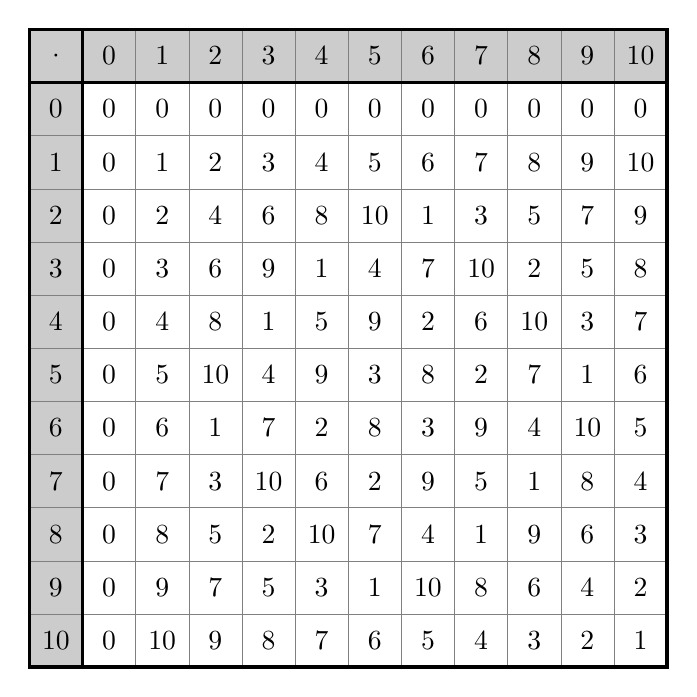
\begin{tikzpicture}[>=latex,thick,scale=0.45]
		\fill[color=gray!40] (0,0) rectangle (18,-1.5);
		\fill[color=gray!40] (0,0) rectangle (1.5,-18);	
		\draw[step = 1.5, gray,very thin] (0,0) grid (18,-18);
		\draw[very thick] (0,0) rectangle (18,-18);
		\draw[very thick] (0,-1.5) -- (18,-1.5);
		\draw[very thick] (1.5,0) -- (1.5,-18);
		\node at (0.75,-0.75) {$\cdot$};
		\foreach \x in {0,...,10}
		\node at (2.25+\x*1.5,-0.75) {$\x$};
		\foreach \y in {0,...,10}
		\node at (0.75,-2.25+\y*-1.5) {$\y$};
		% Row 0
		\node at ( 2.25,-2.25) {$0$};
		\node at ( 3.75,-2.25) {$0$};
		\node at ( 5.25,-2.25) {$0$};
		\node at ( 6.75,-2.25) {$0$};
		\node at ( 8.25,-2.25) {$0$};
		\node at ( 9.75,-2.25) {$0$};
		\node at (11.25,-2.25) {$0$};
		\node at (12.75,-2.25) {$0$};
		\node at (14.25,-2.25) {$0$};
		\node at (15.75,-2.25) {$0$};
		\node at (17.25,-2.25) {$0$};
		% Row 1
		\node at ( 2.25,-3.75) {$0$};
		\node at ( 3.75,-3.75) {$1$};
		\node at ( 5.25,-3.75) {$2$};
		\node at ( 6.75,-3.75) {$3$};
		\node at ( 8.25,-3.75) {$4$};
		\node at ( 9.75,-3.75) {$5$};
		\node at (11.25,-3.75) {$6$};
		\node at (12.75,-3.75) {$7$};
		\node at (14.25,-3.75) {$8$};
		\node at (15.75,-3.75) {$9$};
		\node at (17.25,-3.75) {$10$};
		% Row 2
		\node at ( 2.25,-5.25) {$0$};
		\node at ( 3.75,-5.25) {$2$};
		\node at ( 5.25,-5.25) {$4$};
		\node at ( 6.75,-5.25) {$6$};
		\node at ( 8.25,-5.25) {$8$};
		\node at ( 9.75,-5.25) {$10$};
		\node at (11.25,-5.25) {$1$};
		\node at (12.75,-5.25) {$3$};
		\node at (14.25,-5.25) {$5$};
		\node at (15.75,-5.25) {$7$};
		\node at (17.25,-5.25) {$9$};
		% Row 3
		\node at ( 2.25,-6.75) {$0$};
		\node at ( 3.75,-6.75) {$3$};
		\node at ( 5.25,-6.75) {$6$};
		\node at ( 6.75,-6.75) {$9$};
		\node at ( 8.25,-6.75) {$1$};
		\node at ( 9.75,-6.75) {$4$};
		\node at (11.25,-6.75) {$7$};
		\node at (12.75,-6.75) {$10$};
		\node at (14.25,-6.75) {$2$};
		\node at (15.75,-6.75) {$5$};
		\node at (17.25,-6.75) {$8$};
		% Row 4
		\node at ( 2.25,-8.25) {$0$};
		\node at ( 3.75,-8.25) {$4$};
		\node at ( 5.25,-8.25) {$8$};
		\node at ( 6.75,-8.25) {$1$};
		\node at ( 8.25,-8.25) {$5$};
		\node at ( 9.75,-8.25) {$9$};
		\node at (11.25,-8.25) {$2$};
		\node at (12.75,-8.25) {$6$};
		\node at (14.25,-8.25) {$10$};
		\node at (15.75,-8.25) {$3$};
		\node at (17.25,-8.25) {$7$};
		% Row 5
		\node at ( 2.25,-9.75) {$0$};
		\node at ( 3.75,-9.75) {$5$};
		\node at ( 5.25,-9.75) {$10$};
		\node at ( 6.75,-9.75) {$4$};
		\node at ( 8.25,-9.75) {$9$};
		\node at ( 9.75,-9.75) {$3$};
		\node at (11.25,-9.75) {$8$};
		\node at (12.75,-9.75) {$2$};
		\node at (14.25,-9.75) {$7$};
		\node at (15.75,-9.75) {$1$};
		\node at (17.25,-9.75) {$6$};
		% Row 6
		\node at ( 2.25,-11.25) {$0$};
		\node at ( 3.75,-11.25) {$6$};
		\node at ( 5.25,-11.25) {$1$};
		\node at ( 6.75,-11.25) {$7$};
		\node at ( 8.25,-11.25) {$2$};
		\node at ( 9.75,-11.25) {$8$};
		\node at (11.25,-11.25) {$3$};
		\node at (12.75,-11.25) {$9$};
		\node at (14.25,-11.25) {$4$};
		\node at (15.75,-11.25) {$10$};
		\node at (17.25,-11.25) {$5$};
		% Row 7
		\node at ( 2.25,-12.75) {$0$};
		\node at ( 3.75,-12.75) {$7$};
		\node at ( 5.25,-12.75) {$3$};
		\node at ( 6.75,-12.75) {$10$};
		\node at ( 8.25,-12.75) {$6$};
		\node at ( 9.75,-12.75) {$2$};
		\node at (11.25,-12.75) {$9$};
		\node at (12.75,-12.75) {$5$};
		\node at (14.25,-12.75) {$1$};
		\node at (15.75,-12.75) {$8$};
		\node at (17.25,-12.75) {$4$};
		% Row 8
		\node at ( 2.25,-14.25) {$0$};
		\node at ( 3.75,-14.25) {$8$};
		\node at ( 5.25,-14.25) {$5$};
		\node at ( 6.75,-14.25) {$2$};
		\node at ( 8.25,-14.25) {$10$};
		\node at ( 9.75,-14.25) {$7$};
		\node at (11.25,-14.25) {$4$};
		\node at (12.75,-14.25) {$1$};
		\node at (14.25,-14.25) {$9$};
		\node at (15.75,-14.25) {$6$};
		\node at (17.25,-14.25) {$3$};
		% Row 9
		\node at ( 2.25,-15.75) {$0$};
		\node at ( 3.75,-15.75) {$9$};
		\node at ( 5.25,-15.75) {$7$};
		\node at ( 6.75,-15.75) {$5$};
		\node at ( 8.25,-15.75) {$3$};
		\node at ( 9.75,-15.75) {$1$};
		\node at (11.25,-15.75) {$10$};
		\node at (12.75,-15.75) {$8$};
		\node at (14.25,-15.75) {$6$};
		\node at (15.75,-15.75) {$4$};
		\node at (17.25,-15.75) {$2$};
		% Row 10
		\node at ( 2.25,-17.25) {$0$};
		\node at ( 3.75,-17.25) {$10$};
		\node at ( 5.25,-17.25) {$9$};
		\node at ( 6.75,-17.25) {$8$};
		\node at ( 8.25,-17.25) {$7$};
		\node at ( 9.75,-17.25) {$6$};
		\node at (11.25,-17.25) {$5$};
		\node at (12.75,-17.25) {$4$};
		\node at (14.25,-17.25) {$3$};
		\node at (15.75,-17.25) {$2$};
		\node at (17.25,-17.25) {$1$};
	\end{tikzpicture}
	
\end{center}